%%%%%%%%%%%%%%%%%%%%%%%%%%%%%%%%%%%%%%%%%%%%%%%%%%%%%%%%%%%%%%%%%%%%%
% LaTeX Template: Project Titlepage Modified (v 0.1) by rcx
%
% Original Source: http://www.howtotex.com
% Date: February 2014
% 
% This is a title page template which be used for articles & reports.
% 
% This is the modified version of the original Latex template from
% aforementioned website.
% 
%%%%%%%%%%%%%%%%%%%%%%%%%%%%%%%%%%%%%%%%%%%%%%%%%%%%%%%%%%%%%%%%%%%%%%

\documentclass[12pt]{report}
\usepackage[a4paper]{geometry}
\usepackage[myheadings]{fullpage}
\usepackage{fancyhdr}
\usepackage{lastpage}
\usepackage{graphicx, wrapfig, subcaption, setspace, booktabs}
\usepackage[T1]{fontenc}
\usepackage[font=small, labelfont=bf]{caption}
\usepackage{fourier}
\usepackage[protrusion=true, expansion=true]{microtype}
\usepackage[english]{babel}
\usepackage{sectsty}
\usepackage{url, lipsum}
\usepackage{array,etoolbox}
\usepackage{hyperref}
\usepackage{xcolor}
\usepackage{listings}
\usepackage{minted}
\definecolor{light-gray}{gray}{0.95}

\usepackage{listings}
\usepackage{color}
\def\biblio{\bibliographystyle{apa}\bibliography{References.bib}}
\bibliographystyle{unsrt} % citation and reference list style
\hypersetup{
    colorlinks=true,       % false: boxed links; true: colored links
    linkcolor=black,          % color of internal links (change box color with linkbordercolor)
    % citecolor=green,        % color of links to bibliography
    % filecolor=magenta,      % color of file links
    urlcolor=red           % color of external links
}
%\preto\tabular{\setcounter{magicrownumbers}{0}}
\newcounter{magicrownumbers}
\newcommand\rownumber{\stepcounter{magicrownumbers}\arabic{magicrownumbers}}
\renewcommand\thesection{\arabic{section}}

\newcommand{\HRule}[1]{\rule{\linewidth}{#1}}
% \onehalfspacing
\setcounter{tocdepth}{5}
\setcounter{secnumdepth}{5}
\setcounter{page}{3}


%-------------------------------------------------------------------------------
% HEADER & FOOTER
%-------------------------------------------------------------------------------
\pagestyle{fancy}
\fancyhf{}
\setlength\headheight{15pt}
\fancyhead[R]{Vrije Universiteit Brussel}
\fancyfoot[R]{\thepage}
%-------------------------------------------------------------------------------
% TITLE PAGE
%-------------------------------------------------------------------------------

\begin{document}

\title{ \normalsize \textsc{Cloud Computing and Big Data Processing}
		\\ [2.0cm]
		\HRule{0.5pt} \\
		\LARGE \textbf{\uppercase{RxJS: Twitter popularity tracker app }}
		\HRule{2pt} \\ [0.5cm]
		\normalsize January 12, 2020 \vspace*{5\baselineskip}}

\date{}

\author{
  GEISSER AGUILAR NIKLAUS\\
  \texttt{Niklaus.Geisser@vub.be}\\
  \texttt{0554142}
}

\maketitle
\tableofcontents
\newpage

%-------------------------------------------------------------------------------
% Section title formatting
\sectionfont{\scshape}
%-------------------------------------------------------------------------------

%-------------------------------------------------------------------------------
% Introduction
%-------------------------------------------------------------------------------
\section{Introduction}


\section{Reactive Programming}
Reactive Programming is a paradigm which main approach is to handle continuous time-varying values and propagation of change. It is frequently used in event driven applications since changes in the state are propagated across dependant computations by the execution of the model. Take for instance the sum of two variables (a = 1; b = 2). In the sequential imperative case, the resulting variable will always be 3, even though the values of the variables can change over time. However, in reactive programming, the resulting variable will always be kept up to date, meaning that the application will "react" to the changes of the variables $a$ and $b$ and the sum will be recomputed. This means that all dependant computations will be recomputed when the state changes \cite{BainomugishaEngineer2013Asor}. For instance, it can be said that spread sheets are reactive

\subsection{First class abstraction}
There are two classes of first class abstractions in reactive programming which are behaviours and events.
The term behaviour refers to time-varying or continuous values. Examples of behaviours include timers, mouse position, input field content, etc. On the other hand, events refer to streams of timed or discrete values. For instance, mouse clicks, key presses and asynchronous responses. Events and behaviours are dual to each other \cite{BainomugishaEngineer2013Asor}.

\subsection{Evaluation Model}
The way changes are propagated through the dependency graph in reactive programming is called evaluation model. It is important to identify the actor that will initiate the propagation of changes. In other words, whether the master node will "push" new data to the child nodes (driven by availability) or they will "pull" the data from the master node (driven by demand) \cite{BainomugishaEngineer2013Asor}. These two approaches are called "Pull based" and "Push based" evaluation models. Most cloud computing solutions will use event-push based approaches

\subsection{Glitch avoidance}
Glitches are temporary inconsistencies due to the update propagation order. Glitches can only happen in push based models, meaning that when the source gets new data it propagates it through all dependent computations.  A way to avoid glitches is to arrange expressions in a topologically sorted graph, in that way an expression can only be evaluated after all the others that depend on that one have been evaluated \cite{BainomugishaEngineer2013Asor}.
Most reactive programming languages eliminate glitches by arranging ex- pressions in a topologically sorted graph [Cooper and Krishnamurthi 2006; Meyerovich et al. 2009; Maier et al. 2010], thus ensuring that an expression is always evaluated after all its dependents have been evaluated.

\subsection{Lifting Operation}
The mapping of an operator to a behaviour variant is called lifting. This operation changes a function's type signature and it pushes a dependency graph in the general dataflow of the application.
$f(s) => f_{lifted}(Behaviour<S>)$

\section{RxJS}

ReactiveX is a library for handling asynchronous and event-based programs by making use of observable sequences combining the observer and iterator patterns along with functional programming\cite{reactiveX}.

\subsection{Observer Pattern}
In this pattern, there exists an object called Producer that has a list of listeners or "observers" subscribed to it. Whenever the state of the producer changes, it notifies the listeners by calling their "update" methods \cite{mansilla2018reactive}.

\subsection{Iterator Pattern}
In this pattern, an object is provided to a consumer in order to traverse its contents in an easy way. The interface is composed of two methods: 
\begin{itemize}
  \item \textbf{next()} Gets the next item in the list
  \item \textbf{hasNext()} Check if there is a next item in the list
\end{itemize}
The main objective of the pattern is to encapsulate a traversing logic for different data structures \cite{mansilla2018reactive}.
\subsection{Observable}
The combination of the Observer and Iterator pattern results in another pattern called Rx which is named after the Reactive extension libraries. Observables are a central part of this pattern. They can emit values to consumers when they become available. When a listener or observer is subscribed to an Observable it will receive the values of the sequence whenever the data become available without making a request.

\section{RxJS + ReactJS}
The present project was developed implementing two libraries. ReactJS to build the user interface and RxJS to handle the events and asynchronous flow of the application. Even though this project could have been developed without using a web framework, it is interesting to see how RxJs can be adapted to work within any javascript solution. ReactJS was chosen for two main reasons:
\begin{itemize}
\item Is the second most used library for building UI.
\begin{figure}[h]
\centering
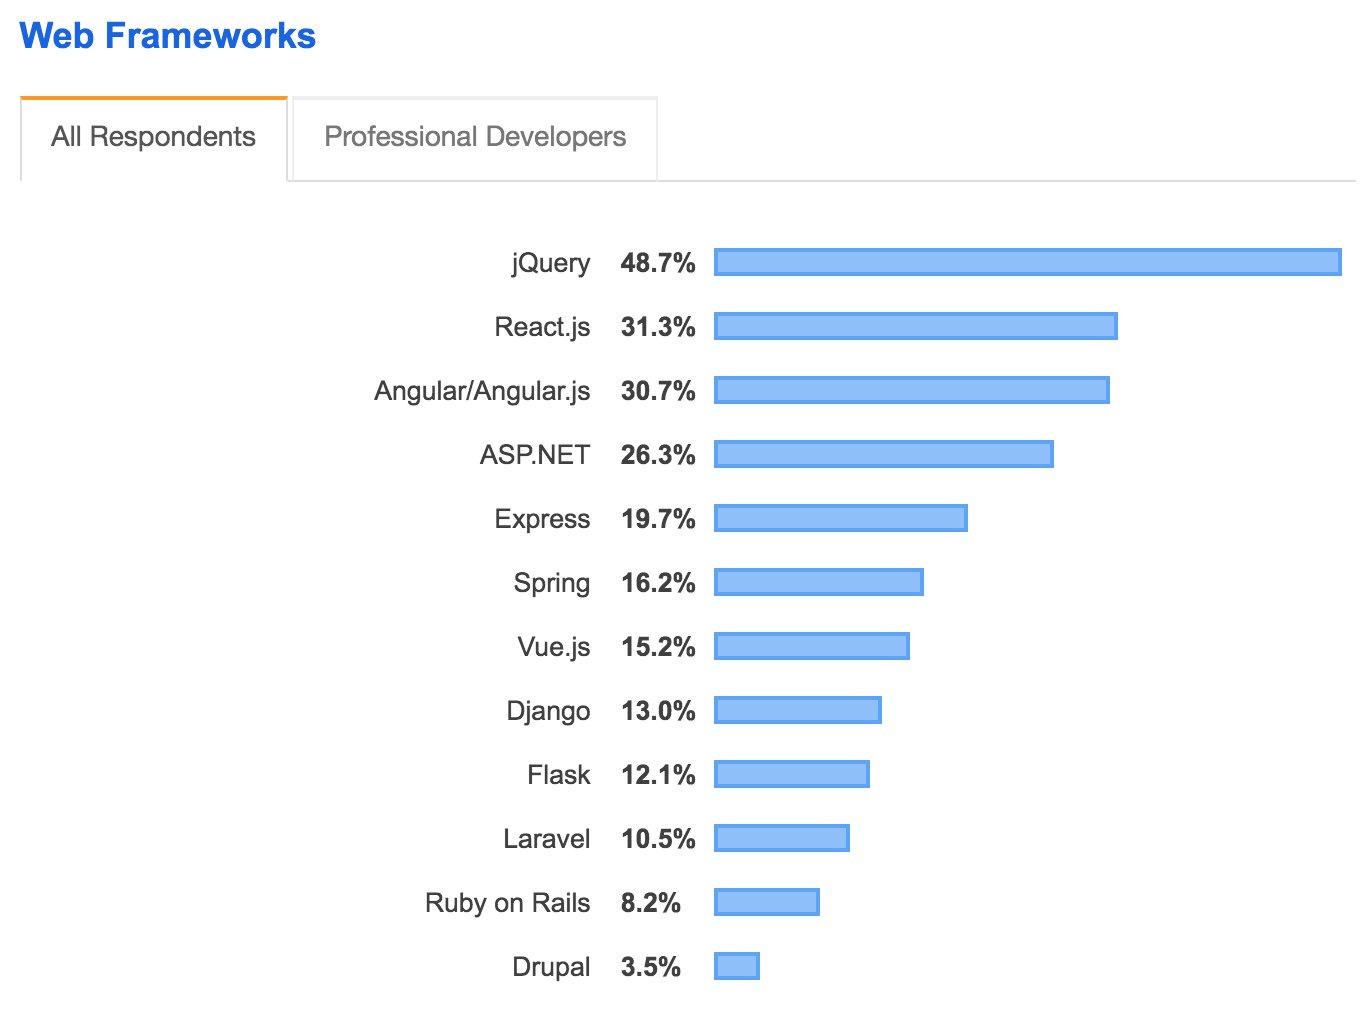
\includegraphics[width=12cm, height=10cm]{react_survey.png}
\caption{StackOverflow developer survey 2019}
\label{fig:stack_react}
\end{figure}
\item It does not come with an integration out of the box of RxJS unlike Angular, thus it makes it a little bit more challenging to join these two libraries.
\end{itemize}

%-------------------------------------------------------------------------------
%Web application section%
%-------------------------------------------------------------------------------

\section{Web application description}
\begin{figure}[h]
\centering
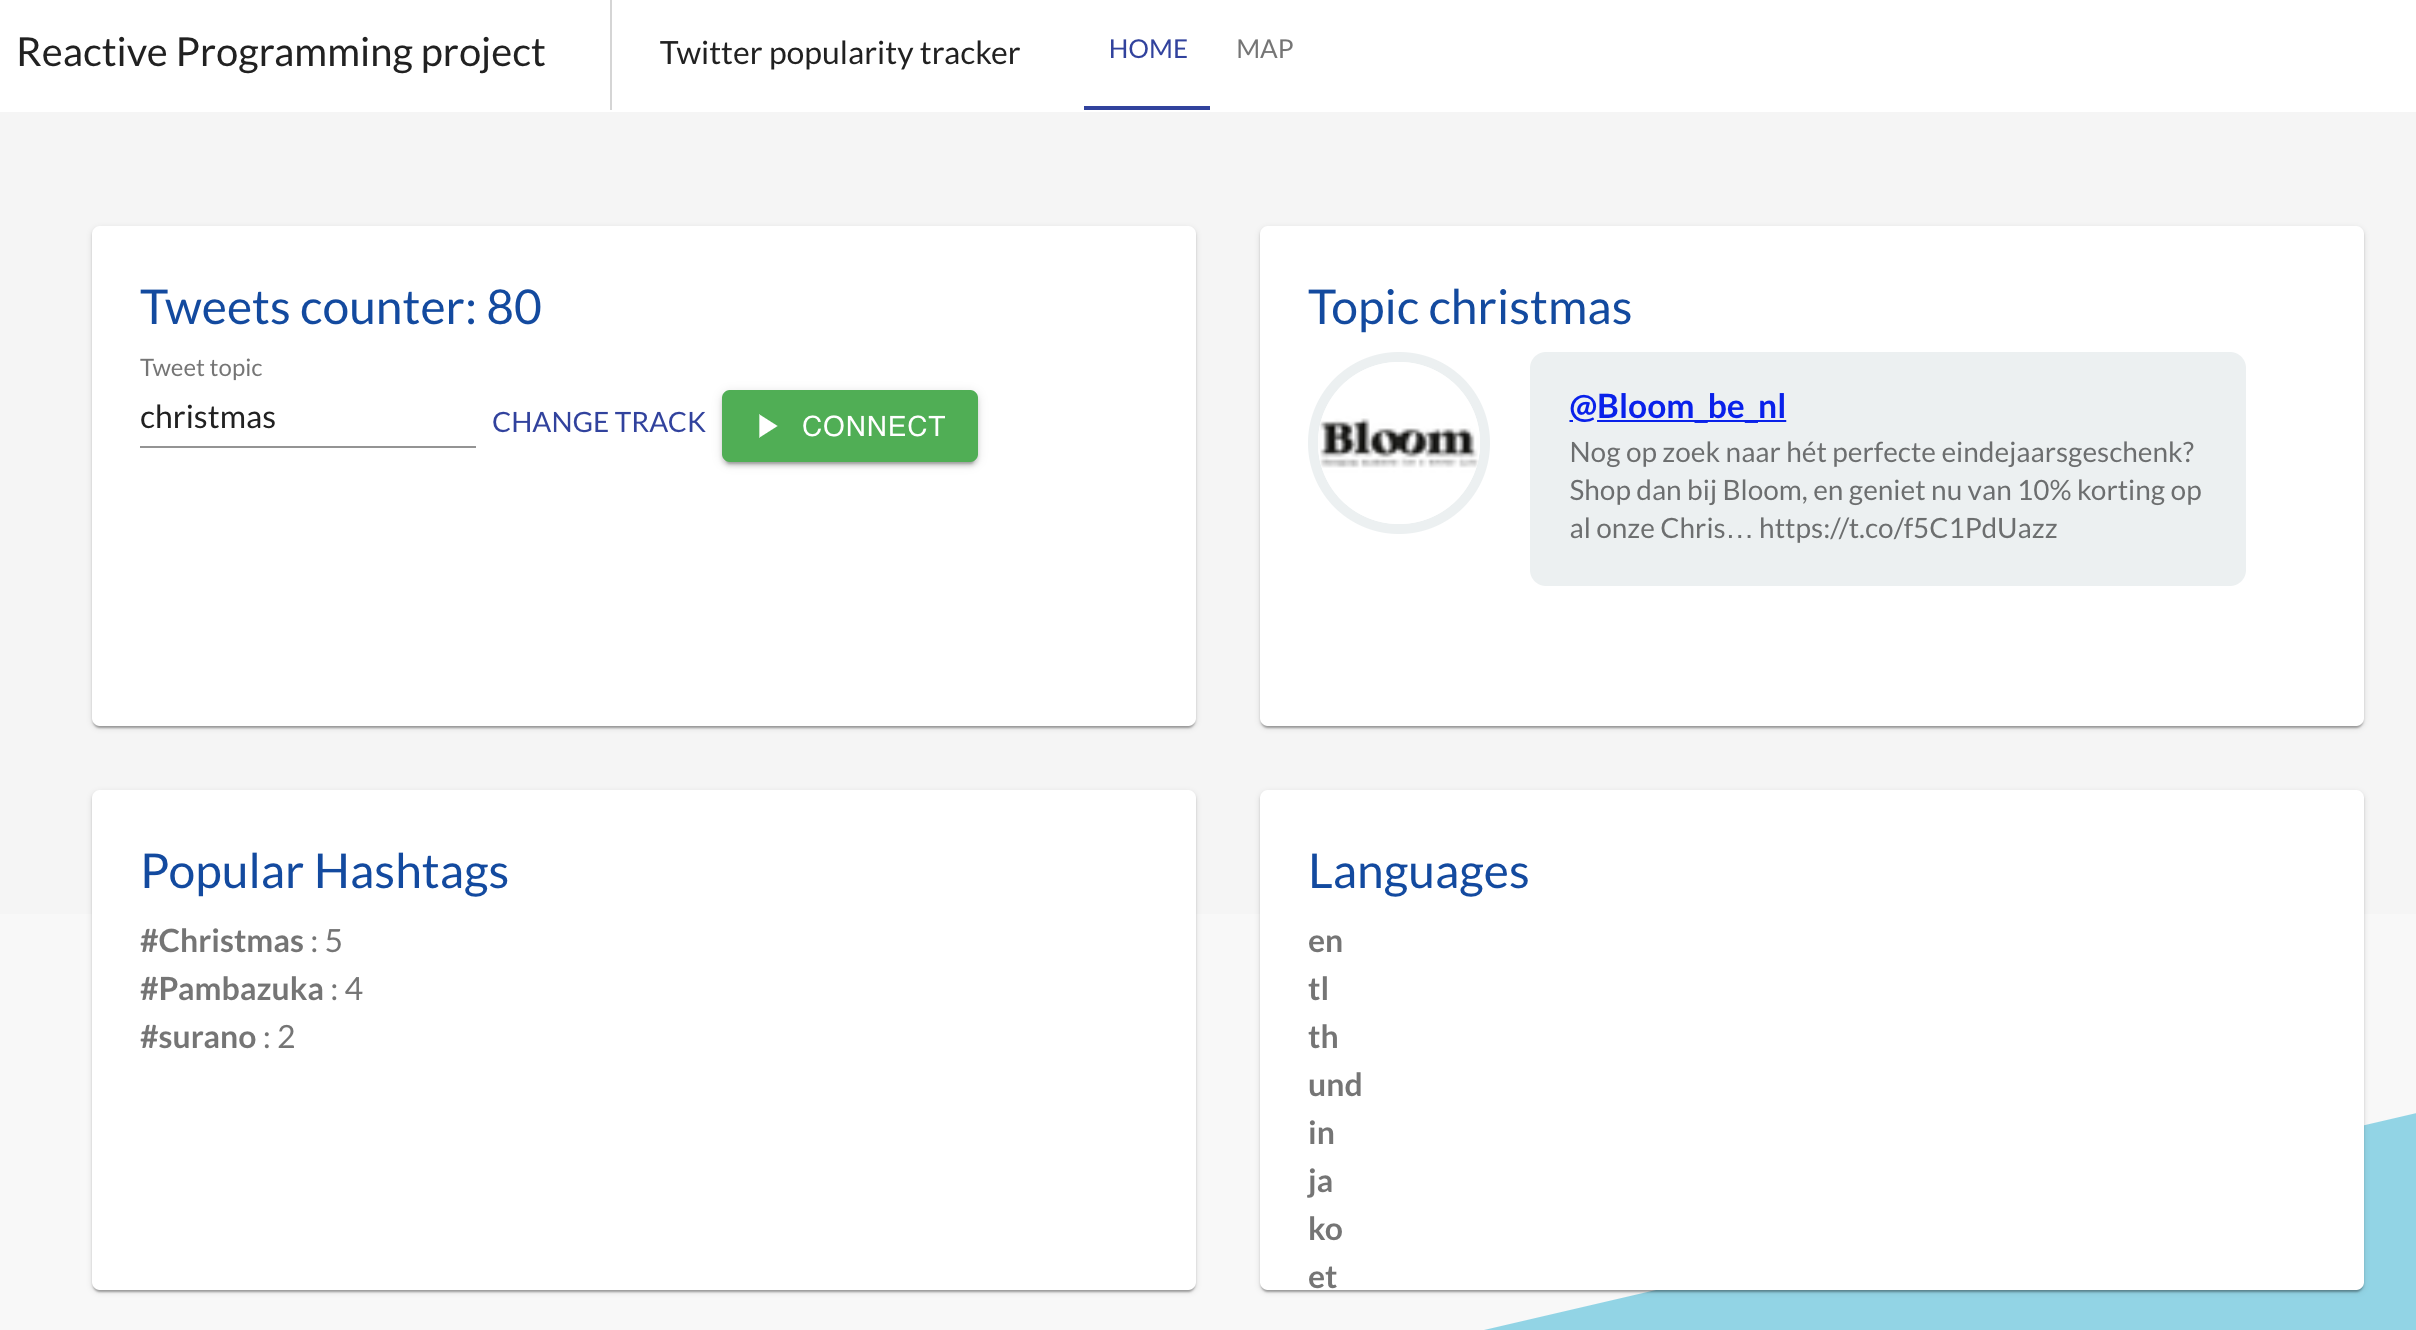
\includegraphics[width=15cm, height=10cm]{main_screen.png}
\caption{Home page of web application}
\label{fig:main_screen}
\end{figure}
\begin{figure}[h]
\centering
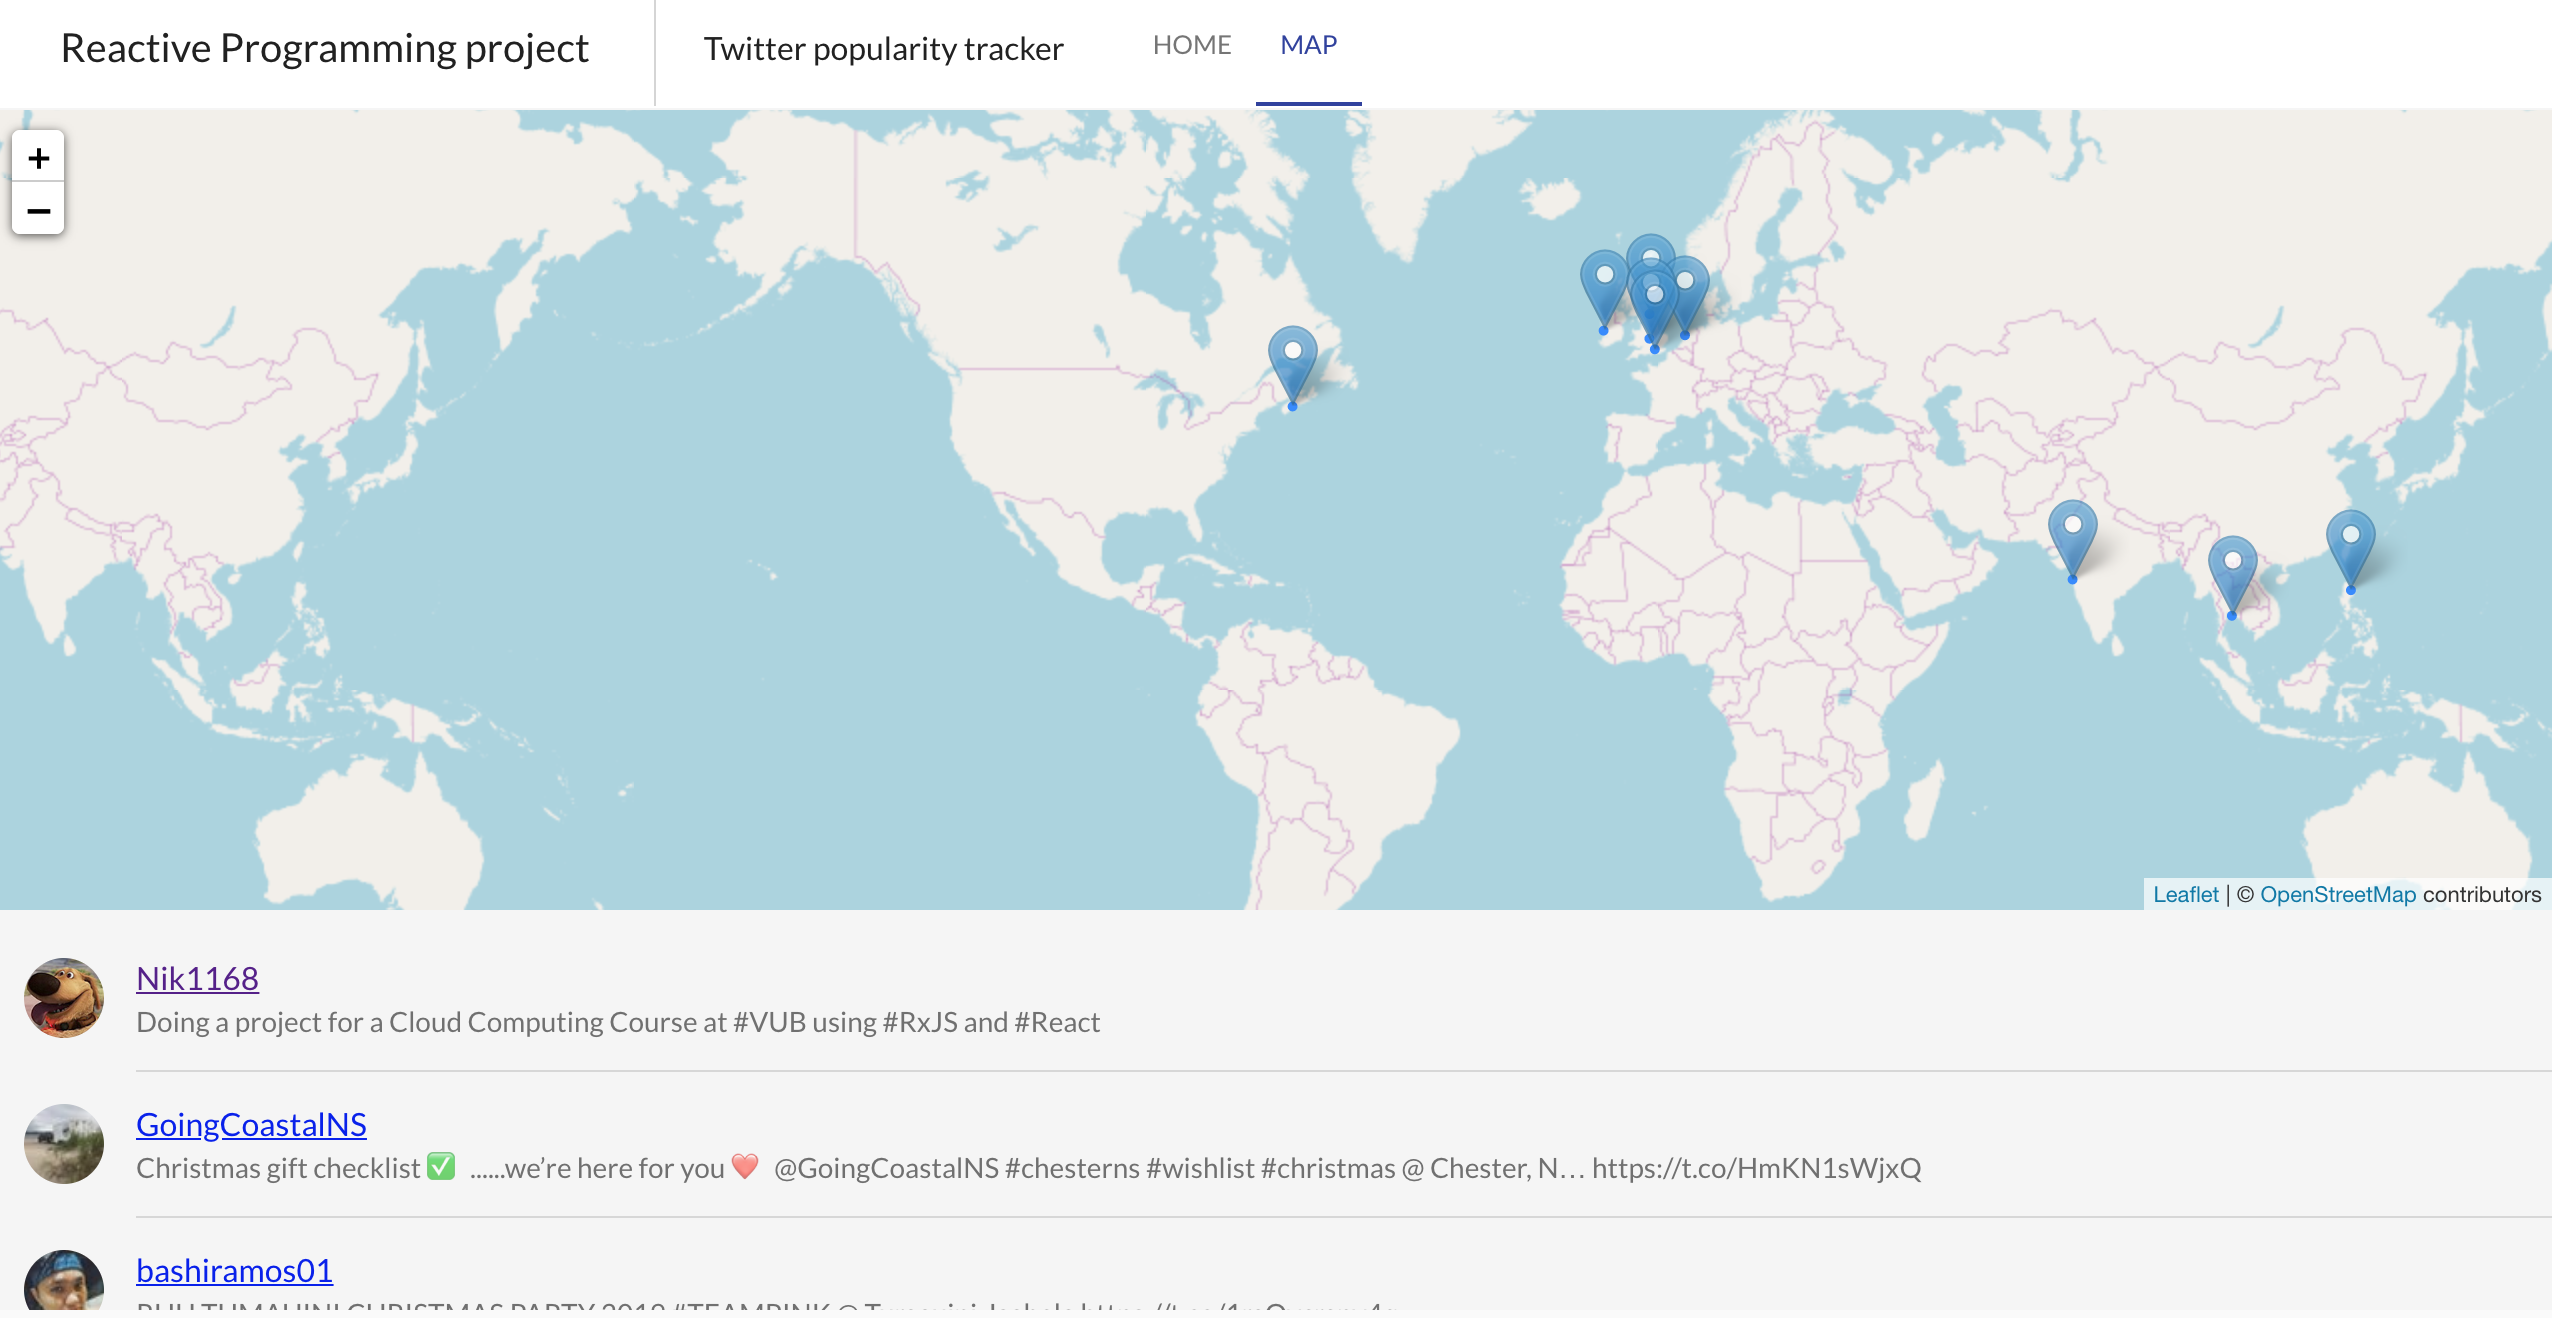
\includegraphics[width=15cm, height=11.2cm]{map_screen.png}
\caption{Map showing location of tweets}
\label{fig:map_screen}
\end{figure}
The web application developed in the present project has the following features that implement several operators of RxJS:
\begin{itemize}
\item A tweet counter that displays the number of incoming tweets in the stream based on a topic.
\item A component that connects to a web socket and let's the user change the topic of the tweets.
\item A component that shows the incoming tweets with a link that takes the user to the actual tweet description in twitter.
\item A component that shows the popular hashtags based on the topic of the tweet stream.
\item A component that lists the distinct languages in which the tweets are written.
\item A component that shows in a map the location of the incoming tweets along with a list displaying them.
\end{itemize}
The backend of the application was implemented in NodeJs using web sockets
%-------------------------------------------------------------------------------
% Description of algorithm
%-------------------------------------------------------------------------------
\section{Implementation}
\subsection{Twitter interaction}
In order to consume the twitter API, it is necessary to apply for a developer account describing what are the use cases intended to use the API. Once the application is approved, one can call the necessary endpoints for the streaming. In particular, the service used is the following:
\href{https://stream.twitter.com/1.1/statuses/filter.json}{https://stream.twitter.com/1.1/statuses/filter.json}, which returns public statuses related to a filter predicate. To consume the service, the following library was used: 
\href{https://www.npmjs.com/package/node-tweet-stream}{https://www.npmjs.com/package/node-tweet-stream}. Additionally, socket.io library was used to handle web sockets communication. Whenever a client connects to a socket in the server we start consuming the streaming. In the frontend side, we declare a Subject (special type of observable that allows values to be multicasted to multiple observer \cite{rxjs}), that will emit the values received by the sockets. 

\begin{minted}[frame=lines,
framesep=2mm,
baselinestretch=1.2,
fontsize=\footnotesize,
linenos]{javascript}
// Front end
let tweetsStream = new Subject();
socket.on('tweet', data => tweetsStream.next(data));
\end{minted}

\begin{minted}[frame=lines,
framesep=2mm,
baselinestretch=1.2,
fontsize=\footnotesize,
linenos]{javascript}
// Backend
io.on("connection", function (socket) {
    t.on('tweet', function (tweet) {
        socket.emit('tweet', tweet);
    });
});
t.track('christmas');
\end{minted}
\subsection{Operators used}
For each of the features of the application, several operators were used that will be described as follows:

\subsubsection{Display tweets}
In order to displays the incoming tweets from the stream, we subscribe to the observable and use a \textbf{debounce} in order to wait a specific amount of time to send each tweet. 
\begin{minted}[frame=lines,
framesep=2mm,
baselinestretch=1.2,
fontsize=\footnotesize,
linenos]{javascript}
tweetsStream
            .pipe(
                debounce(() => timer(50))
            )
            .subscribe((tweet) => {
               // handle list tweets
            })
\end{minted}
Additionally, a request has to be made in order to change the topic of the tweet streaming. In order to do that, we transform the request which is a promise into an observable using the \textbf{from} method from rxJS.
\begin{minted}[frame=lines,
framesep=2mm,
baselinestretch=1.2,
fontsize=\footnotesize,
linenos]{javascript}
export const changeTrack = (track) =>
    from(fetch(`${URL_SERVER}/changeTrack`, {
        method: 'POST',
        headers: {
            'Accept': 'application/json',
            'Content-Type': 'application/json'
        },
        body: JSON.stringify({track})
    })
        .then((res) => res.json()));
\end{minted}

\subsubsection{Tweet counter}
In order to implement the tweet counter we declare an object that will subscribe to the data stream to receive each Tweet.
\begin{minted}[frame=lines,
framesep=2mm,
baselinestretch=1.2,
fontsize=\footnotesize,
linenos]{javascript}
tweetsStream
            .pipe(scan(counter => counter + 1, 0))
            .subscribe(counter => {
                this.setState({count: counter})
            })
\end{minted}
In this case, we use the \textbf{scan} transformation which applies an accumulator over a source Observable \cite{rxjs}. Once the counter is received in the subscription, we can update the state of the component to show it. (Implementation based on practical sessions of the course).

\subsubsection{Popular hashtag tracker}
There are different factors to take into consideration for the implementation of this feature: first of all, not all tweets have hashtags, therefore, we need to perform a filter. (Implementation based on practical sessions of the course)

\begin{itemize}
\item Not all tweets have hashtags, therefore, we need to perform a \textbf{filter}.
\item A tweet can have several hashtags, therefore, in order to get all hashtags we \textbf{map} and transform the array of hashtags into an observable.

\item In order to be able to group the hashtags we use the \textbf{contactAll} operator to pass the subscription of this observable to the next one.

\item Next we use \textbf{groupBy} to group the streams by each hashtag. This operator returns a new grouped observable

\item Once this is done, we apply a \textbf{scan} operator to count the number of occurrences of each hashtag. In order to not list all possible hashtags, we consider a Tweet to be popular if it has more than two occurrences in the stream. It is important to remark that this is a high order observable. 
\end{itemize}

\begin{minted}[frame=lines,
framesep=2mm,
baselinestretch=1.2,
fontsize=\footnotesize,
linenos]{javascript}
tweetsStream
            .pipe(
                filter(tweet => tweet.entities.hashtags.length > 0),
                map(tweet => from(tweet.entities.hashtags)),
                concatAll(), 
                groupBy(hashtag => hashtag.text)
            )
            .subscribe(groupedObservable => {
                groupedObservable
                    .pipe(
                        scan((count, current) => {
                            return {key: current, size: count.size + 1}
                        }, {key: '', size: 0}),
                        filter(res => {
                            return res.size > 1
                        })
                    )
                    .subscribe((result) => {
                        // handle results

                    });
            })
\end{minted}
\subsubsection{Display languages}
To display the languages of the incoming tweets we use the \textbf{distinct} operator since several tweets in the stream have the same language.
\begin{minted}[frame=lines,
framesep=2mm,
baselinestretch=1.2,
fontsize=\footnotesize,
linenos]{javascript}
tweetsStream
            .pipe(distinct(tweet => tweet.lang))
            .subscribe(tweet => {
               // show tweets
            })
\end{minted}
\subsubsection{Map with tweet's location}
In this section, we will show how can we use observables with behaviours, we will use DOM events to change the opacity of a marker in the map by hovering over the list of the respective Tweet. In order to do so, we will use the library react DOM, which has a mouseover event. We create two observables for both events (when hovering or not) and we merge them to make a subscription \cite{mansilla2018reactive}. 
\begin{minted}[frame=lines,
framesep=2mm,
baselinestretch=1.2,
fontsize=\footnotesize,
linenos]{javascript}
tweetsStream
            function isHovering(element) {
        const over = Rx.DOM.mouseover(element).map(identity(true)); ]t
        const out = Rx.DOM.mouseout(element).map(identity(false)); 
        return over.merge(out); 
    }
\end{minted}
To display the tweets in the map we simply make a subscription and filter tweets that have a location. Refer to source code for details of the implementation or go \href{https://fast-bayou-22628.herokuapp.com}{here} to see a live demo.

\section{Run project}
There are two folders called "frontend" and "server". First, install all necessary dependencies in both folders by running \textbf{npm install}. Next start server by entering "server" folder and typping \textbf{npm start}. Do the same for frontend folder. Refer to README file in the source code for more details.

\section{Conclusions}
It can be concluded that RxJS is a powerful tool to deal with asynchronous events and streams of data. It certainly has advantages over promises and callbacks functions. A lot can be done with simple approaches.
\bibliography{References.bib}
\end{document}

